\documentclass[12pt,a4paper]{book}

\usepackage[utf8]{inputenc} % Character encoding
\usepackage[T1]{fontenc}    % Large font encoding
\usepackage{lmodern}        % Latin modern font

\usepackage{hyperref}       % Http links
\usepackage{graphicx}       % Include graphics extension
\usepackage[frenchb,english]{babel} % Typographical rules according to languages

\usepackage{menukeys}       % Include keyboard keys
\usepackage{microtype}      % Better spacing

\usepackage{todonotes}      % Insert todo notes
\usepackage{booktabs}       % Nice tables

\usepackage{fixltx2e}       % Fix few things in latex
\usepackage[american]{isodate} % Date formating with language

\usepackage{comment}        % Comment environement for blocks

\usepackage{array}          % Custom arrays
\usepackage{tabu}           % Avenced arrays
\usepackage{multirow}       % Row merging in tabular
\newcolumntype{C}[1]{>{\centering\arraybackslash}p{#1}}

% \usepackage{nicefrac} % One line fraction
% \usepackage[parfill]{parskip}  % Spaces instead of indentation between paragraphs

\usepackage{listings}	   % Code insertion
\lstdefinestyle{customstyle}{
    basicstyle=\footnotesize,
    breakatwhitespace=false,         
    breaklines=true,                 
    captionpos=b,                    
    keepspaces=true,                                                                                       
    tabsize=4,
    frame=single, %lines
    moredelim=[is][\underbar]{_}{_} % underlines permitted without escape character
}
\lstset{style=customstyle}	
	
\title{ArchPi cheat book}
\author{Jérémy Bardon}
				
\begin{document}
\frontmatter
	\maketitle
	\tableofcontents	

\mainmatter

\chapter*{Preface}
Howto book to learn you a few things you need to know about 
\href{http://archlinuxarm.org/platforms/armv6/raspberry-pi}{ArchLinux ARM} 
on \href{http://www.raspberrypi.org/help/what-is-a-raspberry-pi/}{RPi}. 
From basic setup of the system to side packages installation to turn 
your Raspberry into a music sharing or even a versioning control server.

\section*{Structure of book}
The first part of this book will be focused on system setup and 
basic settings as keyboard language, user account and others. 
The second part will describe how to install some third party sofwares 
as git and mpd server.

\section*{Author words}
I am not an expert in linux system as ArchLinux and even less in electronic 
stuff. However, as a developer I like to tinker with my new toy which is 
a Raspberry Pi. 

I had a lot of troubles when I decided to find uses for it 
and tried to install some third party software. As a result, I am glad to 
write this \og{}book\fg{} to help you to install things on your RPi with ArchLinux.

\chapter{Introduction}
	\section{Are you interested?}
This book is written by a non-specialist of ArchLinux with basic knowledge of 
linux system so I will try to made it as simple as possible for people 
who have no idea about what is console. Indeed, all commands will be 
explained for a better comprehension and an index will be available for you.
\\\\
No matter if you are an expert or a novice, you will be able to find 
how to install stuff on your your Pi plus tips which includes all the problems 
I encounter during my first installation.

	\section{What is a Raspberry Pi}
If you succeed to find this book I guess you allready know but some people 
buy a Raspberry with OpenELEC\footnote{Tiny linux system based on XBMC media center. 
More details on \href{http://openelec.tv}{openelec.tv}} pre-installed so here 
is a little explaination.
\\\\
The Raspberry Pi is a credit-size computer with low performances if you
compare with a common PC. Nevertheless, it means its power consumption is
very low (1W for B+ version\footnote{Most robust version of RPi with 512MB 
of RAM and 4 usb ports}) so it is not a problem to let it on forever. 
\newpage
\begin{figure}[h]
	\centering
	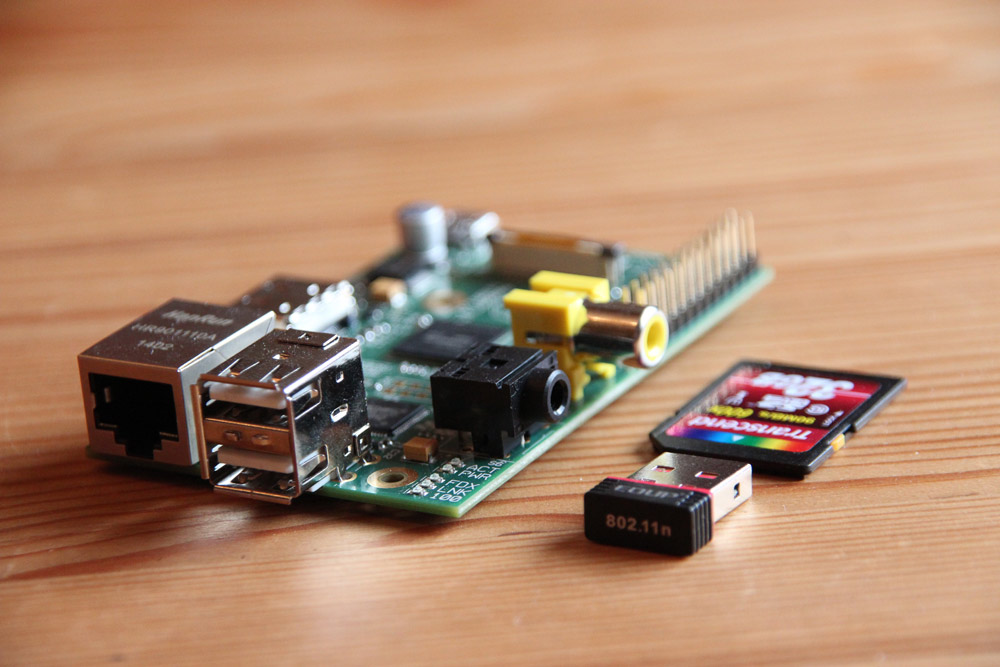
\includegraphics[scale=0.2]{images/RaspberrySize.jpg}
	\caption{Raspberry Pi B+}
	\label{figure:RaspberrySize}
\end{figure}

Finally if you install a good linux distribution on it you can turn this old computer
into a cheap server on which you will have the control. You can use it 
at home for file sharing, media player or others but it is also possible
to host a website which will be available on the internet\footnote{An example
of website hosted by a Rpi on \href{http://raspberrypi.goddess-gate.com}
{raspberrypi.goddess-gate.com}}.

	\section{ArchLinux versus \href{http://www.raspbian.org}{Raspbian}}
	\label{section:ArchVsRaspbian}
The operating system recommended by the Raspberry fundation is Raspbian -- a custom version of the famous Debian\footnote{One of the most popular linux 
system. See \href{https://www.debian.org/intro/about}{debian.org} for more details} system -- optimized for RPi hardware. 
\\\\
In general it will be the default choice for an inexperienced user to get
a user interface and most common softwares allready installed at the first boot.
However we forget the limited performances of the Raspberry and you will be able to realize that for yourself if you decided to install Raspbian. 
\\\\
A server does not need a user interface except a terminal which is enough 
to manage it everyday from anywhere. As a result, my choice has been focused 
on ArchLinux which is a pretty light and fast system. In addition, system 
updates are based on rolling release \footnote{Definition on \href{http://
en.wikipedia.org/wiki/Rolling\_release}{wikipedia/Rolling\_release}} model, 
so it means you do not have one version of the system. You will just receive 
updates frequentely -- as soon as their availability -- and it will be not 
necessary to reboot during the upgrade process.

%\documentclass[12pt,a4paper]{book}\usepackage{hyperref}\usepackage[english, frenchb]{babel}\begin{document}
\chapter{ArchLinux installation}
\section{We are \textsc{Noobs}}
There are two ways to install ArchLinux on a Raspberry Pi: the first is 
the ArchLinux way -- no idea if it is the same with other systems -- and 
the second is an official manager which works with many systems.

\begin{itemize}
	\item follow instructions from archlinuxarm.org\footnote{Specific 
		  instruction on \href{http://archlinuxarm.org/platforms/armv6/
		  raspberry-pi}{archlinuxarm.org/platforms/armv6/raspberry-pi}} but 
		  you need to have a linux system
		  
	\item use \textsc{Noobs}, an operating system install manager provided by 
		  the Raspberry fundation\footnote{Details on \href{http://
		  www.raspberrypi.org/help/noobs-setup}{www.raspberrypi.org/help/
		  noobs-setup}}\\
\end{itemize}

I choose \textsc{Noobs} because it is the easiest way to install a
system on a RPi and in addition you get an extra \og{}boot manager\fg{} which 
is usefull. Moreover, you can complete the full setup of your SD card on any 
system by following the RPi website guide.
\\\\
\textsc{Noobs} is available on two forms: one for offline installation 
and the other -- the smallest one -- downloads automatically the last release 
of the system online. The offline installer contains many systems -- which 
takes a large space -- but you can just keep ArchLinux and remove others 
(in \texttt{os} folder). Anyway, you need to know that other systems files 
will be keeped after the installation so it is loose space. If you still want 
to use the offline way because you have no choices, you will have to find  
an older version of \textsc{Noobs} because ArchLinux has been removed since  
the last release.

\section{Installer usage}
% wifi ou ethernet

%\end{document}

%\documentclass[12pt,a4paper]{book}\usepackage[utf8]{inputenc}\usepackage[T1]{fontenc}\usepackage{lmodern}\usepackage{hyperref}\usepackage{graphicx}\usepackage[english, frenchb]{babel}\usepackage{listings}	\lstdefinestyle{customstyle}{basicstyle=\footnotesize,breakatwhitespace=false,breaklines=true,captionpos=b,keepspaces=true,tabsize=4,frame=single}\lstset{style=customstyle}\usepackage{menukeys}\begin{document}
\chapter{Basic setup}

\section{Change language}
There are no default languages selected in ArchLinux but the keyboard map is set to 
qwerty\footnote{Most common layout for keyboards} at the beginning. To choose 
your language you have to complete two steps and then the system will be able to 
use it for characters encoding and some softwares as \texttt{nano}.

\subsection{Enable yours}
Before choosing yours it is necessary to enable it in \texttt{/etc/locale.gen}
file with \texttt{locale} tools. 

You will need to use \texttt{nano} to edit the configuration file -- \keys{\ctrl 
+ W} can help you to search -- and remove \og\#\fg{} before the language you want 
to enable (fr\_FR.UTF-8 for example), to save your changes press \keys{\ctrl + X}.
\\
\begin{lstlisting}[language=bash,caption=Enable your language]
$ locale # Current language settings

# Edit the /etc/locale.gen file
$ nano /etc/locale.gen

$ locale-gen # Update available languages
$ locale -a  # See available languages
\end{lstlisting}

\subsection{Change your settings}
The second step is to set the language and configure your keyboard map. 
Notice that you will have to logout for the system to take into account 
changes you made with language setup.
\\ 
\begin{lstlisting}[language=bash,caption=Change language settings]
$ localectl status
  System Locale: n/a  # System language
      VC Keymap: n/a  # Virtual console
     X11 Layout: n/a  # Graphic interface
     
# Change system language (enabled one)
$ localectl set-locale LANG=fr_FR.UTF-8

# List of keymaps, choose the one you want "fr-pc" for example
$ localectl list-keymaps

# Change settings 
# no-convert not update VC with X11 and vice versa
$ localectl set-keymap --no-convert fr-pc     # VC Keymap
$ localectl set-x11-keymap --no-convert fr-pc # X11 Layout

# Logout to apply changes
$ exit
\end{lstlisting}

\section{Configure wifi connexion}
\subsection{Check your dongle}
The first thing you can do is check if your dongle has been recognized by 
the system and can be used.

\begin{lstlisting}[language=bash,caption=Check wifi device]
$ ifconfig -a wlan # All wireless interfaces (also disabled)

# If you see a line with "wlan0" try to enable it
$ ip link set wlan0 up

# If you see again "wlan0" your dongle is working
# Disable it after the check
$ ifconfig wlan # Without -a show only enabled interfaces
$ ip link set wlan0 down
\end{lstlisting}

There are a lot of ways to connect your RPi to a network using a wifi dongle 
but all of them requires to install a package before -- wifi-menu needs 
dialog, iw and wpa\_supplicant are not installed -- so it is necessary to 
use an ethernet wire to begin.

\begin{lstlisting}[language=bash,caption=Install wireless dependencies]
# pacman is the package manager in ArchLinux
#        -S install a new package 
#
# dialog to get wifi-menu interface
# wpa_supplicant for wireless network protected with wpa keys
#
$ pacman -S dialog wpa_supplicant
\end{lstlisting}

\subsection{Searching the internet}
Once you installed all the packages -- synonym for software -- that wifi-menu 
needed to run you can launch it with \og{}\texttt{wifi-menu}\fg{} command.

\begin{figure}[h]
	\centering
	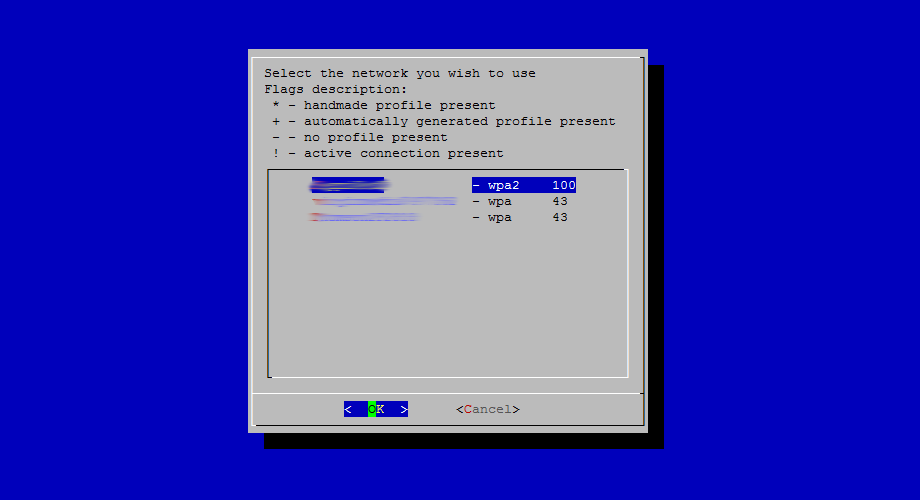
\includegraphics[scale=0.3]{images/WifiMenu.png}
	\caption{wifi-menu interface}
	\label{figure:WifiMenu}
\end{figure}

Then, select your network -- with \keys{\arrowkeyup} and \keys{\arrowkeydown} -- 
, type your password (if required) and you will be connected to your wireless 
network.
\newpage
\section{Create yourself}
\subsection{Simple user}
The default username and password for ArchLinux are \texttt{root/root}, this 
user got all right on the system it means he can do anything -- even break 
the system -- so it is not recommanded to use it.
\\
\begin{lstlisting}[language=bash,caption=Create a new user called jeremy]
$ useradd -m jeremy # Creates user jeremy and his home folder
$ passwd jeremy     # Changes jeremy password
\end{lstlisting}

Now we have a new user account for everydays usage. You can see all users on 
your system with \og{}\texttt{cat /etc/passwd}\fg{} which will display the 
content of the config file for users.

\subsection{Very important user}
It is possible to specify user rights with \texttt{visudo} command, the general syntax for one user is 
the following \og{}\texttt{username machine=(targetuser) commands}\fg{}, 
let's look at some details:


%# Attribute rights with a specific format
%$ visudo
%# Add new line: "jeremy ALL=(ALL) ALL"

\begin{description}
\item[username] name you gave to \texttt{useradd} command
\item[machine] machine on where rights are applied, ALL in general
\item[target user] user that we takes the rights
\item[command] allowed commands separated with one coma -- no spaces --, 
use exclamation mark for banned commands
\end{description}

%\end{document}

\documentclass[12pt,a4paper]{book}\usepackage{array}\usepackage{multirow}\newcolumntype{C}[1]{>{\centering\arraybackslash}p{#1}}\usepackage{multirow}\usepackage[utf8]{inputenc}\usepackage[T1]{fontenc}\usepackage{lmodern}\usepackage{hyperref}\usepackage{graphicx}\usepackage[english, frenchb]{babel}\usepackage{listings}	\lstdefinestyle{customstyle}{basicstyle=\footnotesize,breakatwhitespace=false,breaklines=true,captionpos=b,keepspaces=true,tabsize=4,frame=single,moredelim=[is][\underbar]{_}{_}}\lstset{style=customstyle}\usepackage{menukeys}\begin{document}
\chapter{Web server}
\section{Nginx versus Apache}
In web servers world there are three major actors: Apache, nginx and 
IIS (by Microsoft). If you look at the number of production uses\footnote{Netcraft 
survey available on \href{http://news.netcraft.com/archives/2014/02/03/february-
2014-web-server-survey.html}{news.netcraft.com/archives/2014/02/03/february-2014-
web-server-survey.html}} you will see that I followed the distribution from above 
it means \textasciitilde{}55\% for our old Apache and \textasciitilde{}15\% for 
the two others.
\\\\
However, it appears like Apache decreases by 5\% and nginx get these same 5\% all 
that between January 2014 and February 2014. Now, I can tell you I choosed to use 
nginx instead of Apache for some reasons and the nginx rise is one of them.
\\\\
Let's sum up some advantages and drawbacks of using nginx instead of apache. Few 
of them are extracted from raspbian-france.fr\footnote{Article on the same topic 
(in french), see \href{http://raspbian-france.fr/installer-nginx-raspbian-
accelerez-serveur-web-raspberry}{raspbian-france.fr/installer-nginx-raspbian-
accelerez-serveur-web-raspberry}} but others are personnal. 
\\\\
\begin{table}
\label{table:AvantagesNginx}
\centering
	\begin{tabular}{C{1cm}|p{9cm}}
		\multirow{4}{*}{+} 
		& Asynchronous server\footnote{Parallel execution of tasks}\\
		& More scalable\footnote{Ability to support a lot of connexions in one time}\\
		& Less RAM usage (think about our poor RPi)\\
		& Config file syntax (XML vs readeable)\\
		\hline
		\multirow{4}{*}{-} 
		& Less mature (1995 vs 2004)\\ 
		& Some PHP behaviours may differ from Apache\\
		& .htacess not work directly with nginx\\
	\end{tabular}
	\caption{Advantages and drawbacks of nginx}
\end{table}

\section{Installation}
To run a non-static website, nginx is not sufficient we also need to install PHP 
-- for dynamic pages -- and a mySQL database to save our precious data. In 
addition, we will install phpMyAdmin which a tool -- written in PHP -- to manage 
a mySQL database through a web interface. 

\begin{lstlisting}[language=bash,caption=Install a full web server]
# php-fpm is the nginx module for PHP
# mariadb is a mySQL database
$ pacman -S nginx php-fpm mariadb phpmyadmin

# Enable and run services
$ systemctl enable nginx php-fpm mysqld
$ systemctl start nginx php-fpm mysqld
\end{lstlisting} 

Nginx server works well but php is not enabled in configuration files. Moreover, 
there are some incompatibilties troubles in initial setup.

\begin{lstlisting}[language=bash,caption=Enable php in nginx]
# First problem: welcome file directory is not set in
# availables directories for php
#
# Update php config file
# Search open_basedir, add ":/usr/share/nginx/html/" at the end
#
$ nano /etc/php/php.ini

# Second problem: php not enabled and contains bad setup
# in nginx configuration file
#
# Uncomment (remove #) on the following block and change it 
# to fit the example
#
$ nano /etc/nginx/nginx.conf

# pass the PHP scripts to FastCGI server listening on 127.0.0.1:9000
#
location ~ \.php$ {
    root   /usr/share/nginx/html; # Fix path to php files

# Use sockets   
#   fastcgi_pass   127.0.0.1:9000; 
    fastcgi_pass   unix:/var/run/php-fpm/php-fpm.sock;
            
    fastcgi_index  index.php;

# Use fastcgi.conf file
#   fastcgi_param  SCRIPT_FILENAME  /scripts$fastcgi_script_name;
#   include        fastcgi_params;
    include        fastcgi.conf;
}
\end{lstlisting}

The last thing to do is enabling mysql extensions in php configuration files to 
be able to perform SQL queries on local database through php scripts.
\begin{lstlisting}[language=bash,caption=Enable php in nginx]
$ nano /etc/php/php.ini

# Remove ";" before mysql and mysqli extensions
;extension=mysql.so
;extension=mysqli.so
\end{lstlisting}

Each time you change nginx or php configuration files you have to reload and 
restart the corresponding service for it to take into account your changes.
\begin{lstlisting}[language=bash,caption=Reload and restart a service]
# Restart only considered service
$ systemctl reload nginx php-fpm 
$ systemctl restart nginx php-fpm
\end{lstlisting}

\section{Basic verifications}
The next step is to check our web server with basic verifications to test whether
the installation worked well. We will simply try to access to the default nginx 
page remotely, create a php page and display it and finally access to local 
database. 

\subsection{Nginx and php}
During installation process, nginx places a welcome page called \emph{index.html} 
in \texttt{/usr/share/nginx/html} directory. However Php gives no sample to test 
with nginx therefore we will create a new php script in welcome page directory.
\\\\
The content of this new script will simply display php configuration on 
your server.
\lstset{language=php,caption=Php simple script}
\lstinputlisting{code/index.php}

The goal of these test is to access to \emph{index.html} and \emph{index.php} 
from a remote web browser to check if nginx and php work well on your server. 
\\\\
To perform that, type the IP address of your RPi on your PC web browser -- 
followed by /index.html and then /index.php -- and you will see nginx welcome page 
and php config respectively.

\subsection{MySQL}
% 2 things : mysql and mysql + php
\begin{lstlisting}[language=bash,caption=Test mySQL installation]
$ mysql -uroot    # Connect to local database with root user
> show databases; # List of databases
> use mysql;      # Go into mysql database
> show tables;    # List of tables in current database

# Perform SQL query to list users
> select host, user, pasword from user;
> exit; # Logout from local database

# If nothing works try to launch mysql install script
# user: user account used by mysql service
# ldata: path to MariaDB data directory
# basedir: path to MariaDB installation directory
$ mysql_install_db --user=mysql --ldata=/var/lib/mysql 
    --basedir=/usr
\end{lstlisting}

\section{Set custom directory}
Nginx default setup set this directory as the root of 
your server but websites are usually hosted in \texttt{/var/www} so I will explain 
you how to move the welcome page into that new file.

\begin{lstlisting}[language=bash,caption=Move nginx welcome page]
# Create /var/www directory and move into it
$ cd /var
$ mkdir www # Create a folder named "www"
$ cd mkdir

# Copy directory (with -r) source destination
$ cp -r /usr/share/nginx/html/ /var/www/

# Move a directory but if source and destination
# are in same directory rename source
$ mv /var/www/html /var/www/home
\end{lstlisting} 

Before trying to access to your website it will be necessary to configure nginx 
and php for the new path. The sample nginx configuration file contains some 
help to do specific things so we will save it and create a new one with the 
following example.

\begin{lstlisting}[language=bash,caption=Configure nginx and php]
# Save and change nginx file
$ mv /etc/nginx/nginx.conf /etc/nginx/nginx.conf.old
$ nano /etc/nginx/nginx.conf # See following example

# Update php config file
# Search open_basedir and add ":/var/www/" at the end
$ nano /etc/php/php.ini

# Do not forget to reload and restart services
\end{lstlisting} 
\lstset{language=bash,caption=nginx configuration}
\lstinputlisting{code/nginx.conf}

% /usr/share/webapps/phpMyAdmin
% link + enable + nginx config
% domain
\end{document}

%\documentclass[12pt,a4paper]{book}\usepackage{array}\usepackage{tabu}\usepackage{multirow}\newcolumntype{C}[1]{>{\centering\arraybackslash}p{#1}}\usepackage{multirow}\usepackage[utf8]{inputenc}\usepackage[T1]{fontenc}\usepackage{lmodern}\usepackage{hyperref}\usepackage{graphicx}\usepackage[english, frenchb]{babel}\usepackage{listings}	\lstdefinestyle{customstyle}{basicstyle=\footnotesize,breakatwhitespace=false,breaklines=true,captionpos=b,keepspaces=true,tabsize=4,frame=single,moredelim=[is][\underbar]{_}{_}}\lstset{style=customstyle}\usepackage{menukeys}\begin{document}
\chapter{Jukebox}
\section{Do I need that?}
Maybe you want to use your Raspberry as a jukebox controlled remotely, so your 
music will be played on sound devices -- through HDMI or DVI port -- attached to 
your RPi.
\\\\
A MPD\footnote{MPD for Music Player Daemon} server is exactly what you need and in 
addition it can manage playlists -- not explained here -- and it exists a plenty 
of applications\footnote{A list of client are available on mpd wiki, see 
\href{http://mpd.wikia.com/wiki/Clients}{mpd.wikia.com/wiki/Clients}} which are 
dedicated or compatible with. 
\\\\
In following sections you will learn how to setup your server and then you will 
discover four clients for various platforms (PC and smartphones).

\section{MPD setup}\label{section:MpdSetup}

There are two things you need to take care of when you want to install a mpd 
server: how to play music on the RPi and where your music will be stored. 
\\\\
In the example, it is a \og{}classic\fg{} situation wherein you music is located 
in a folder called \emph{music} placed in a user home directory.

\begin{lstlisting}[language=bash,caption=Install mpd server]
# mpd is the server
# alsa-utils manage your RPi audio outputs
#
$ pacman -S mpd alsa-utils

# Update the mpd config file to work with
# the RPi audio (see the next example)
$ nano /etc/mpd.conf

# Mpd files (including music database) are located
# in /var/lib/mpd so you have to change it's owner
# for the mpd user to be able to access it
#
# chown: change file or diretory owner
# "mpd:mpd": new owner (user and his group)
#
$ chown mpd:mpd /var/lib/mpd

# My music is located in the SD card, where the system
# is installed: /home/jeremy/music
#
# In default configuration, your home directory can only 
# be crossed by you but the mpd user must access to your
# music inside
#
# chmod: changes rights on a file or a directory
# o+x: anyone can cross the specified directory
# or execute the file (if it is a file)
#
$ chmod o+x /home/jeremy
\end{lstlisting} 

\lstset{language=bash,caption=Mpd configuration file,label=listing:MpdConfigFile}
\lstinputlisting{code/mpd.conf}

A RPi has two audio outputs (HDMI and DVI) so you can play your music on your 
screen (or TV, or audio system plugged in your TV) and in a headset or any device 
which provides a jack input. 
\\\\
Do not forget the power of a Raspberry, is modularity can help you to setup 
bluetooth or airplay wireless network to play your music. However, these 
interesting solutions will be not covered in this book.
\\
\begin{lstlisting}[language=bash,caption=Set audio output]
# Set audio output to HDMI
# Last number: 0 (auto, avoid it), 1 (DVI), 2 (HDMI)
$ amixer cset numid=3 2

# Fix HDMI troubles
# Uncomment hdmi_force_hotplug=1 and hdmi_drive=2
$ nano /boot/config.txt

# You must reboot for HDMI changes
$ reboot

# Enable, start and then check if the service started
$ systemctl enable mpd
$ systemctl start mpd
$ systemctl status mpd
\end{lstlisting}

\section{Music directory on usb device}
\subsection{Connect an usb device}
Connect a device to an linux system as ArchLinux is called \emph{mount}, once you
connected you device the system will be able to see it with no ways to access it.
\\\\
It is after the \emph{mount} operation that the system get an access to the device 
and programs as mpd will be able to read on.

\begin{lstlisting}[language=bash,caption=Mount an external device]
# List of connected devices
$ fdisk -l
# One device: mmcblk0, zero because you can have others sd cards 
# called mmcblk1, mmcblk2, ...
Disk /dev/mmcblk0 : 7,5 GiB, 8017412096 bytes, 15659008 sectors

# Divided in 2 parts (partitions)
# Note: this table was truncated in lines and columns
Device          Size    Id  Type
/dev/mmcblk0p1  116,2M   e  W95 FAT16 (LBA)
/dev/mmcblk0p2    7,3G  85  Linux extended

# Create a directory in /mnt where you
# will see your device files
$ mkdir /mnt/sdcard

# Mount a device (mmcblk0 for example)
#
# Can add some options:
# -t ntfs-3g: format type of the device
# -o uid=user,gid=group: owner of mounted directory
#
$ mount /dev/mmcblk /mnt/sdcard

# Unmount a device: use the target directory
# choosed on mounting operation
#
# Some devices may be used by programs or services
# Be careful you are not in your device directory (use pwd)
#
$ umount /mnt/sdcard

# List mounted directories
$ mount
/dev/sda1 on /mnt/hd1 type vfat 
\end{lstlisting}

If you use some devices with a Windows system they are maybe formated with the 
\emph{ntfs} format that is not recognize by default on a linux based system.
\\\\
To solve this trouble you have to install \emph{ntfs-3g} which contains 
necessary drivers and an easiest way to mount ntfs devices.
\begin{lstlisting}[language=bash,caption=Mount ntfs devices]
# Install the package with ntfs drivers
$ pacman -S ntfs-3g

# For ntfs-3g works you need to reboot
$ reboot

# Mount your ntfs device
# Short for "mount -t ntfs-3g /dev/mmcblk /mnt/sdcard"
$ ntfs-3g /dev/mmcblk /mnt/sdcard
\end{lstlisting}

\subsection{Change directory in mpd}
To change your music directory in MPD this is only one file to update 
mpd.conf (refer to \ref{listing:MpdConfigFile}) which contains the path to your 
music on \emph{music\_directory} line.
\\\\
Nevertheless, this is one thing you need to take care of: rights on every directory 
in your path. In linux system, there are three access types : read, write and 
execute knowing execute means \og{}can cross\fg{} for directories.

\begin{lstlisting}[language=bash,caption=Analyze rights on home]
$ ls -l / | grep home
drwxr-x--x  3 root root  4096 18 dec.  23:48 home
\end{lstlisting}

Let's analyze the previous result for \texttt{/home} directory to 
able to understand rights easily.

\begin{table}[h]
\centering
	\begin{tabu}{p{2cm}|p{40px}|l|l|p{40px}|l|p{2cm}}
		\rowfont{\bfseries\footnotesize}
		Rights (modes) & Links number & Owner & Group & Size (in bytes) & Last update   & Folder name\\
		&&&&&&\\
		\rowfont{\ttfamily\small}
		drwxr-x--x     & 3            & root  & root  & 4096            & 18 dec. 23:48 & home\\
	\end{tabu}
	\caption{Details on \texttt{ls -l} syntax}
\end{table}

Now, we can decrypt \texttt{ls -l} results and identify who is the owner of a 
file and of which group it belongs. With the first part of the output it is 
possible to deduce what things a user can do on the given file.

\begin{table}[h]
\centering
	\begin{tabular}{rl}
		\hline
		\multicolumn{2}{|c|}{Indicators}\\
		\hline
		d   & File type: directory (d), symbolic link (l), file (-)\\
		&\\
		\hline
		\multicolumn{2}{|c|}{Rights -- nothing(-) read(r) write(w) execute(x)}\\
		\hline
		rwx & Owner, got all rights usually\\ 
		r-w & Users who belongs to group\\ 
		--w & Others\\ 		
	\end{tabular}
	\caption{Rights on a file}
\end{table}

Remember, the initial purpose was to change our mpd music directory so let's 
change the directory to \og{}\texttt{/home/jeremy/music}\fg{} with good rights 
to ensure the \emph{mpd} user will be able to access to the \emph{music} directory 
and read files into.

\begin{lstlisting}[language=bash,caption=Check rights on path]
# We want to check that mpd user can acces
# to /home/jeremy/music, we have to check the three directories
#
$ ls -l / | grep home

# Anyone can cross home: OK
drwxr-xr-x  3 root root  4096 18 dec.  23:48 home

$ ls -l /home | grep jeremy
# Nobody can cross this directory exept jeremy: NOT OK
drwx------ 4 jeremy jeremy 4096 30 dec.  11:56 jeremy

# Add execute right for everyone because mpd do not 
# belongs to jeremy group
#
# Format: level+/-right
#   level: u (owner), g (owner group), o (anyone)
#   +/-: + to add right, - to remove it
#   right: r (read), w (write), x (execute)
#
$ chmod o+x /home/jeremy

$ ls -l /home | grep jeremy
# Anyone can cross this directory: OK
drwx-----x 4 jeremy jeremy 4096 30 dec.  11:56 jeremy

$ ls -l /home/jeremy/ | grep music
# Anyone can read music files into this directory: OK
drwxr-xr-x 2 jeremy jeremy 4096 29 dec.  12:18 music

# Now the full path has been verified: mpd can cross each
# directories from root and read in music folder
\end{lstlisting}

\section{Classic and web clients}

There many mpd clients available and it is necesarry to distinguish thoses which 
are installed on the server -- as web clients -- and others that are on a remote 
machine owned by the client.

\subsection{External clients}
I will present you two applications which are mpd client and as much as possible 
multiplatform or at least compatible with most common devices.
\\\\
The first one is \texttt{MPDroid} an Android application available on the play 
store\footnote{Download MPDroid on the play store at \href{http://play.google.com/
store/apps/details?id=com.namelessdev.mpdroid}{play.google.com/store/apps/details?
id=com.namelessdev.mpdroid}} which enable you to manage your mpd server depending 
on the wireless network you are connected.
\\\\
GMPC\footnote{Gnome music player client} is the second client that I will talk 
about because it's strong point is that it is multiplateform so compatible with 
Windows, Mac OSX and Linux systems.
\\\\
To setup the connexion between your application and the mpd server on the RPi the 
only thing you need is it's IP address or domain name. That is why we did not 
change the default port -- 6600 -- and set a password to access it but feel free 
to do it if it is necessary for you.

\subsection{YMPD web client}
YMPD is a lightweight and easy to install web client interface build over the 
bootstrap. It means the interface is really responsive and it can be used 
either on the PC or on a smartphone through a web browser.

\begin{lstlisting}[language=bash,caption=ympd setup]
# wget: tool to download files from network
$ pacman -S wget

# Use wget to download ympd release
$ wget http://www.ympd.org/downloads/ympd-1.2.3-armhf.tar.bz2

# Unpack ympd from the downloaded archive
$ tar -xvf ympd-1.2.3-armhf.tar.bz2

$ rm ympd-1.2.3-armhf.tar.bz2 # Remove unused archive
$ mv ympd /usr/bin            # Move executable to the "classic" directory

# Run ympd server and choose the port you will
# use to connect to it
$ ympd --webport 2020 # Any port > 1024
\end{lstlisting}

Now, you can connect to the ympd web interface from any web browser access to 
\href{http://RPiIP:2020}{http://RPiIP:2020} but pay attention to use the port 
you choosed when you launched ympd your server.

\subsection{Ampache}
If you are looking for a more complex and customizable solution for your mpd 
server web client, Ampache can be the answer to your problem.
\\\\
It is php based application (similar to phpMyAdmin) which allows you to manage 
music catalogs  -- on your server and on remote machines -- and play them on the 
server or locally in your browser (with streaming).

\begin{lstlisting}[language=bash,caption=Download Ampache]
# You will need unzip to unpack ampache 
$ pacman -S unzip

# Download last ampache release
$ wget https://github.com/ampache/ampache/archive/develop.zip

# Unpack ampache, remove zip file and rename ampache directory
$ unzip develop.zip 
$ rm develop.zip
$ mv ampache-develop ampache

# Create a domain with nginx by using the following
# config file (too long but necessary) available at :
# http://github.com/ampache/ampache/wiki/Installation#nginx
#
# See Subdomains and site setup in Web server chapter of this book
# if you have some troubles
\end{lstlisting}

Ampache offers a php script called \emph{install.php} that you can reach by going 
to \href{http://RPiIP/install.php}{http://RPiIP/install.php} but in my case it 
allways redirect me to \emph{/test.php} which tells me that I do not respect 
prerequires.
\\\\
Finally, once I launched install script after some setup, I have realized that 
pretty much all things I have done before had to be done by this script. 
\\\\
As a result either you are lucky and the install script works or follow me for 
some setup to fill requirements and tell to the install script to do nothing 
because we have done it's work.

\begin{lstlisting}[language=bash,caption=Ampache setup]
# The test page show me 6 errors at the begin
# here are the "name" of theses tests plus the 
# ways to pass them

# MySQL and PHP iconv extension
# Problem: php extensions not enabled
#
# Remove ";" before: extension=pdo_mysql.so
#                     extension=iconv.so
#
$ nano /etc/php/php.ini
$ systemctl reload php-fpm

# Configuration file readibility and validity
# Problem: wrong name for ampache config file
#
$ cd /usr/share/webapps/ampache/config
$ mv ampache.cfg.php.dist ampache.cfg.php

# Database connexion
# Problem: user account for database not set in 
# ampache configuration file
#
# Fill following fields with right values
# (remember you may changed the root password)
#        database_username = root
#        database_password = password
#
$ nano /usr/share/webapps/ampache/config/ampache.cfg.php


# Database table
# Problem: ampache database and tables not created
#
$ mysql -u root -ppassword # no space between -p and password
> create database ampache;
> use ampache;
> source /usr/share/webapps/ampache/sql/ampache.sql;
> exit
\end{lstlisting}

At this point, Ampache let you run the install script but it says some tests about 
the configuration files fails, ignore them and then skip database and configuration 
file steps. The last thing to do is creating an admin account to connect yourself 
to ampache web client.

\section{Bluetooth notes}
\begin{lstlisting}[language=bash,caption=Bluetooth]
$ pacman -S bluez bluez-utils
\end{lstlisting}
%\end{document}

\documentclass[12pt,a4paper]{book}\usepackage{array}\usepackage{tabu}\usepackage{multirow}\newcolumntype{C}[1]{>{\centering\arraybackslash}p{#1}}\usepackage{multirow}\usepackage[utf8]{inputenc}\usepackage[T1]{fontenc}\usepackage{lmodern}\usepackage{hyperref}\usepackage{graphicx}\usepackage[english, frenchb]{babel}\usepackage{listings}	\lstdefinestyle{customstyle}{basicstyle=\footnotesize,breakatwhitespace=false,breaklines=true,captionpos=b,keepspaces=true,tabsize=4,frame=single,moredelim=[is][\underbar]{_}{_}}\lstset{style=customstyle}\usepackage{menukeys}\usepackage{comment}\begin{document}
\chapter{Git server}
\section{Why would you use Git}
For some reasons, you need to keep several versions of documents so you make 
copies -- can be long and space consumer -- but it still difficult to get the 
last version when more than one person works on the same document.
\\\\
Git is a versionning tool which can do this work for you and in addition keep 
traces of who modified what on each document in a project. This tool will be not  
intrusive and can be used at every moments of a projet -- even if it is allready 
started -- it ensure that you have a project which is the \og{}good version\fg{} 
everytime and it is up-to-date.
\\\\
Largely used in programming projects it can be usefull for any types of projects 
which contains files readable by a simple text editor. You can get an idea of what 
is git by browsing projects on \href{http://github.com}{github.com} which is the 
most famous git projects host because it is free for public (open source) projects.

\section{Install Git and add projects}
To visualize git projects on web interface the first thing you need to have is a 
git project. In order to create our own projet we will download an existing one 
to have a real history and some things to visualize. 
\\\\
I choose to use an open source project -- Firefox OS\footnote{Firefox OS is the 
operating system developed by the Mozilla foundation for smartphones. More 
informations on \href{https://www.mozilla.org/en-US/firefox/os/}{www.mozilla.org/
en-US/firefox/os/}, sources availables on \href{https://github.com/mozilla/
firefox-ios}{github.com/mozilla/firefox-ios}} -- because it is quite fast to 
download and have some folders with enough commits to be interesting.

\begin{lstlisting}[language=bash,caption=Install git and add projects]
# Install git package
$ pacman -S git

# Create repositories(projects) directory
$ mkdir /srv/git

# Get an existing project on github to test our web 
# interface, Firefox OS in this example.
$ cd /srv/git
$ git clone https://github.com/mozilla/firefox-ios.git
\end{lstlisting}

There are a few directories that are most used for repositories but I retained two 
of them: \texttt{/home/git/} and \texttt{/srv/git/}. 
\\\\
In ArchLinux, websites and ftp are by default in \emph{/srv}, and \emph{/home/git} 
is the home directory for \emph{git} user -- which is not a physic user -- so to 
keep a kind of consistency -- in my opinion -- I prefer the second alternative. 

\section{Host repositories}
\subsection{Create a new project}
Host a git project is quite easy because it is really close from creating a local 
git repository. You just must think about adding \emph{--bare} option to specify 
that your project is not a working copy. 
\begin{lstlisting}[language=bash,caption=Create a repository on your server]
# Let's create a new git project called "project"
# Naming convention: add .git at the end of your project name
# to specify it is not a working copy
#
$ mkdir /srv/git/project.git
$ cd /srv/git/project.git
$ git init --bare # --bare: not a working copy
\end{lstlisting}

On a remote machine on which you want to work, clone the project and do a first 
commit on your project.
\begin{lstlisting}[language=bash,caption=Clone repository to work]
# Clone project
# username is your username for local account on the server 
$ git clone username@RPiIP:/srv/git/project.git

# Create a new file and commit
$ cd project
# New file called README.md with "New project" text inside
$ echo "New project" > README.md 
$ git commit -am"First commit"
$ git push origin master # First time, after just "git push"
\end{lstlisting}

\subsection{Use an existing project}
If you want to host a git project which allready exists it is possible to do. 
There two possible situations:
\begin{itemize}
	\item The project is allready hosted by someone else or websites like GitHub 
		  or BitBucket.
	\item It is a local project so hosted locally
\end{itemize}

\subsubsection{Allready hosted}
As you can imagine, the first situation is the easier to solve, you just have to 
clone the repository from the server with a specific option.

\begin{lstlisting}[language=bash,caption=]
$ git clone username@RPiIP:/srv/git/project.git --bare
\end{lstlisting}

Note that the folder you will get will be named \emph{project.git} so it is not a 
working copy. In addition, notice that is the same \emph{--bare} option as when 
you create a new repository on the server.

\subsubsection{Local project}
The first thing to do is retrieve the local project on the server. There are many 
ways to it, I advice to use FTP -- if you setup an FTP -- but for others here is 
a simple way if you have a linux system.

\begin{lstlisting}[language=bash,caption=]
# Your project is named project
$ scp username@RPiIP:/srv/git /local/path/to/project
\end{lstlisting}

With the working copy on your server, the last thing to do is clone the repository 
as \emph{bare} locally and remove the working copy.

\begin{lstlisting}[language=bash,caption=Host repository from local copy]
# Extract project informations
$ git clone --bare /srv/git/projet /srv/git/project.git
$ rm -r /srv/git/project
\end{lstlisting}
% Change remote ?
	
% Different from clone apparently
\begin{comment}
	\begin{lstlisting}[language=bash,caption=Host repository from local copy]
# Extract project informations
$ mv /srv/git/project/.git /srv/git/project.git
$ rm -r /srv/git/project

# Declare repository as bare
$ cd /sr	v/git/project.git
$ git config --bool core.bare true
	\end{lstlisting}
\end{comment}
\section{Web application for viewing}
\subsection{GitWeb: Build-in solution}
Gitweb is the web interface offered by git when you install it. Based on cgi 
technology, it is a bit slow but very refined so easy to use and understand.
\\\\
You can see a live usage of git web at \href{http://repo.or.cz/w?a=project\_list}
{repo.or.cz/w?a=project\_list}, browse projets, commit and all things you want and 
before abandoning GitWeb keep in mind that we will improve a little bit the visual 
aspect.

\subsubsection{Installation and configuration}
\begin{lstlisting}[language=bash,caption=Gitweb setup]
# Gitweb is a cgi script, you need to install 
# some packages
$ pacman -S fcgiwrap spawn-fcgi

# Update php configuration to accept .cgi files
$ nano /etc/php/php-fpm.conf
# Uncomment and add .cgi
security.limit_extensions = .php .php3 .php4 .php5 .cgi

# Set your repositories folder in gitweb.conf
# Look at the next example
$ nano /etc/gitweb.conf  # Is created of not exist
\end{lstlisting}

\lstset{language=bash,caption=gitweb.conf file}
\lstinputlisting{code/gitweb.conf}

\subsubsection{Configure nginx and install cgi tools}
According to the ArchLinux wiki, it is necessary to change the \emph{fcgiwrap.service} 
file because it uses spawn-fcgi so trust the wiki. Note you have to restart 
fcgiwrap service after your updates.

\lstset{language=bash,caption=fcgiwrap.service from wiki.archlinux.org/index.php/gitweb}
\lstinputlisting{code/fcgiwrap.service}

The standard subdomain file presented before will not work in this case because 
gitweb does not contains php scripts but only one cgi script.

\lstset{language=bash,caption=Gitweb configuration for nginx}
\lstinputlisting{code/gitweb}

\subsubsection{Finishing touch}
After that, you will be able to access to your gitweb interface with the domain 
you defined -- \texttt{gitweb.local.pi} in the example -- but if do not see any 
projects although you set some of them in the directory you specified in 
\emph{gitweb.conf}, try to launch git daemon.

\begin{lstlisting}[language=bash,caption=]
$ /usr/lib/git-core/git-daemon --inetd --export-all --base-path=/srv/git
\end{lstlisting}

\mbox{}\\\\
The last thing you can do is replace the default theme the one developed by 
kogakure\footnote{More informations on his web site: \href{http://kogakure.github
.io/gitweb-theme/}{kogakure.github.io/gitweb-theme/}} which is a little bit more 
appealing.

\begin{lstlisting}[language=bash,caption=Install kogakure gitweb theme]
# Save default theme
$ cp -r /usr/share/gitweb/static/ /usr/share/gitweb/static.old

# Retrieve kogakure theme, copy it in right folder
# and delete unused files
$ git clone https://github.com/kogakure/gitweb-theme.git
$ cp gitweb-theme/git* /usr/share/gitweb/static
$ rm -r gitweb-theme
\end{lstlisting}

\subsection{GitList: Simple GitHub clone}

If you are looking for a git web interface which look like GitHub -- with less 
side features -- GitList is probably a good alternative for you. 
\\\\
This project is hosted by GitHub at \href{https://github.com/klaussilveira/gitlist}
{github.com/klaussilveira/gitlist} but as said in the README file, do not clone 
the repository and prefer download the packaged version on the GitList website at 
\href{http://gitlist.org}{gitlist.org}.

\begin{lstlisting}[language=bash,caption=Download GitList]
# Download
$ cd /usr/share/webapps
$ wget https://s3.amazonaws.com/gitlist/gitlist-0.5.0.tar.gz

# Extract and remove unused files
$ tar -xvf gitlist-0.5.0.tar.gz
$ rm gitlist-0.5.0.tar.gz
\end{lstlisting}

Let's declare a new subdomain for GitList, a sample is available in it's directory 
-- \texttt{/usr/share/webapps/gitlist/INSTALL.md} -- but here I will propose you 
a shorter solution. Note you have to use at least one of these two sample because 
GitList uses url rewriting.

\lstset{language=bash,caption=GitList configuration for nginx}
\lstinputlisting{code/gitlist}

Now you can access to GitList interface but you may have some errors messages and 
your are forced to fix these troubles.

\begin{lstlisting}[language=bash,caption=Fix GitList troubles]
# Message 1
# The "/usr/share/webapps/gitlist/cache" folder must be writable 
# for GitList to run.
#
$ mkdir /usr/share/webapps/gitlist/cache # If not exist
$ chown http:http /usr/share/webapps/gitlist/cache

# Message 2
# Please, create the config.ini file.
$ cd /usr/share/webapps/gitlist/
$ mv config.ini-example config.ini

# Message 3
# Please, edit the config file and provide your repositories directory
# Solution: set repositories[] = '/srv/git/'
#
$ nano /usr/share/webapps/gitlist/config.ini
\end{lstlisting}

\section{Gitolite: manage projects}

In the case wherein you have few repositories and you do not need to 
setup access constraints the git common usage will be sufficient.
\\\\
However, if you are looking for a tool which enables you to restrict 
access to repositories for specific persons -- or even groups --  
gitolite is the answer to your problem.
\\\\
The documentation for gitolite is available at \href{http://gitolite.com}
{gitolite.com} and it is well written and understandable. During 
your research may be you found a similar tool called \emph{gitosis} 
which is the ancestor of gitolite. It appears that gitosis is no longer 
used and developped so that why I choose to install gitolite.

\subsection{Installation}

Gitolite will use \emph{git} user and functionalities so it is 
to install git first. In this configuration I made the choice to 
store git repositories -- and gitolite configuration -- in 
\texttt{/srv/git} which will be the home directory of \emph{git} 
user.

\begin{lstlisting}[language=bash,caption=Gitolite installation]
# Download and install gitolite
$ cd /tmp
$ git clone git://github.com/sitaramc/gitolite
$ gitolite/install -to /bin
$ rm -r gitolite

# Create git user directory
$ mkdir /srv/git
$ chown git:git /srv/git

# Set /srv/git as git use home
# Add path, the line for git user should looks like :
#     git:x:997:997:git daemon user:/srv/git:/bin/bash
$ nano /etc/passwd
\end{lstlisting}

A this point, gitolite has been installed but it not yet usuable. 
The last thing to do is defining the administrator which will be able 
to manage repositories access through the \emph{gitolite-admin} 
repository.
\\\\
Interactions with the git server will be made through ssh with the 
git user. As a result, the only way to authenticate users is with 
their ssh public key, so we first need to get that key in order 
to define the administator for gitolite.

\begin{lstlisting}[language=bash,caption=Get ssh public key and define gitolite administrator]
# On administrator machine

# Generate key, press enter for each questions
$ ssh-keygen -t rsa

# Copy ssh public key to the server as admin.pub
$ scp ~/.ssh/id_rsa.pub jeremy@local.pi:/srv/git/admin.pub

# On the server as git user
# Connect and configure administrator
$ ssh git@RpiIP
$ cd /srv/git
$ gitolite setup -pk admin.pub
\end{lstlisting}

Once the administrator set in gitolite configuration, you will be able to access 
to the configuration repository from the administrator machine. 
\\\\
By default two repositories are created -- gitolite-admin and testing -- the 
first contains the configuration for gitolite and the second is empty because it 
will allows you to test your access for different users.
 
\begin{lstlisting}[language=bash,caption=Gitolite administration]
# On administrator machine
$ git clone ssh://git@RPiIP/gitolite-admin

# Contains repositories names and rights for users
$ nano gitolite-admin/conf/gitolite.conf

# admin user have all access on gitolite-admin
repo gitolite-admin
    RW+     =   admin

# admin user will be able to pull but not to push
repo testing
    R       =   admin # here remove W
    
# Commit and push changes to update gitolite configuration
$ git commit -am"Restrict testing access for admin user"
$ git push
\end{lstlisting}

Now the administrator user have all rights on \emph{gitolite-admin} repository, he
can pull \emph{testing} project but gitolite will denied push operations. Gitolite 
allows you to define groups of users as described in the GitHub repository
\footnote{Gitolite repository at \href{https://github.com/sitaramc/gitolite}
{github.com/sitaramc/gitolite}} so here these features will be not explained.
\\\\
As mentioned before, the documentation is well written and I want you to pay 
attention at this particular page\footnote{Article of the gitolite documentation 
about settings troubles available at \href{http://gitolite.com/gitolite/emergencies.html}
{gitolite.com/gitolite/emergencies.html}} which describes some process to follow 
in case of emergencies, for example if you lost administrator public key.

% Uninstall > http://gitolite.googlecode.com/git-history/f023591183365980d11c1ba352461bea9863746f/doc/uninstall.html
\subsection{Setup repositories}
\subsection{Adapt GitWeb and GitList}


\end{document}

%\documentclass[12pt,a4paper]{book}\usepackage{array}\usepackage{tabu}\usepackage{multirow}\newcolumntype{C}[1]{>{\centering\arraybackslash}p{#1}}\usepackage{multirow}\usepackage[utf8]{inputenc}\usepackage[T1]{fontenc}\usepackage{lmodern}\usepackage{hyperref}\usepackage{graphicx}\usepackage[english, frenchb]{babel}\usepackage{listings}	\lstdefinestyle{customstyle}{basicstyle=\footnotesize,breakatwhitespace=false,breaklines=true,captionpos=b,keepspaces=true,tabsize=4,frame=single,moredelim=[is][\underbar]{_}{_}}\lstset{style=customstyle}\usepackage{menukeys}\usepackage{comment}\begin{document}
\chapter{Download box}
Many people uses their servers as seed boxes -- for torrent -- or an intermediate 
to download their files faster because a server has an high speed connexion. 
Considering you RPi will be behind you internet connexion it will be totally useless 
for us.
\\\\
However it allows you to download big files -- for torrent with poor sources -- 
without leaving your PC switched on all night and the RPi is a very low energy 
consumer. In addition combined with an FTP or a file sharing system all your 
downloads will be accessible for other people on your network.

\section{Direct download with aria2}
aria2 is download manager which is able to handle http an torrent links. It is 
very easy to use with it's command line interface but we will add a web interface 
at the top of it to manage our downloads remotely from any web browser.

\begin{lstlisting}[language=bash,caption=Aria2 setup]
$ pacman -S aria2

# Download directory with access rights
$ mkdir /srv/downloads 
$ chmod o+w /srv/downloads

# Create configuration file with new example
$ nano /etc/aria2.conf
\end{lstlisting}

The configuration file can be set in any directory because you can specify to 
aria2 which file to use for it's configuration. In this example, this file is 
stored into \texttt{/etc} directory because it mostly contains configuration 
files but you can put it in your home directory.

\lstset{language=bash,caption=Aria2 configuration file}
\lstinputlisting{code/aria2.conf}

Now, you can use aria2 with it's command line interface but we will install the 
web interface before testing it and specify the configuration file directory.

\begin{lstlisting}[language=bash,caption=Install aria2 interface]
# Retrieve last release and put it in the usual directory
$ cd /usr/share/webapps/
$ git clone https://github.com/ziahamza/webui-aria2.git

# Create nginx domain or use this dirty way
$ ln -s /usr/share/webapps/webui-aria2/ /usr/share/nginx/html/aria2

# Setup and start a new service to run aria2 as a daemon
# See next example 
$ nano /usr/lib/systemd/system/aria2.service
$ systemctl start aria2

# You can try to download this image: 
# http://www.mumbly58.fr/wp-content/uploads/2013/01/archlinux-logo.png
$ ls /srv/downloads # must see image after download complete
\end{lstlisting}

Our web interface is directly connected to the aria2 program which have to be 
launched at every moment. Especially when you want to see your downloads through 
the web interface and even if they are stopped.
\\\\
Create a service which runs aria2 is the designated solution to complete this 
kind of tasks so here is an example.

\lstset{language=bash,caption=Run aria2 as a service}
\lstinputlisting{code/aria2.service}

\section{Torrent with rtorrent}

The previous software -- aria2 -- can handle torrents downloading like rtorrent 
but the second is dedicated and provides a very comfortable interface in the 
console. 
\\\\
I do not know what are the technical differences but if you want not 
use a web interface for torrents, rtorrent is the best solution in my opinion.

\subsection{rTorrent installation}
\begin{lstlisting}[language=bash,caption=rTorrent installation]
$ pacman -S rtorrent

# Torrents directory
$ mkdir /srv/torrent
$ chmod o+w /srv/torrent

# Session directory for rtorrent operations
$ mkdir /tmp/rtorrent
$ chmod o+w /tmp/rtorrent

# rTorrent configuration file, change the following options
# according to the two directories you created before
#
# directory = /srv/torrents
# session = /tmp/rtorrent
#
$ cp /usr/share/doc/rtorrent/rtorrent.rc ~/.rtorrent.rc
\end{lstlisting}

Considering there are no indications about how to use the rtorrent interface, I 
will the main commands to use for your torrents management.

\begin{table}[h]
\centering
	\begin{tabular}{lp{9cm}}
		\keys{\return} & Select torrent file to add (use \keys{\tab} to see current 
					 directory files)\\
					 
		\keys{\arrowkeyup} and \keys{\arrowkeydown} & Switch between seleced 
					 torrent\\
					 
		\keys{\arrowkeyright} & Visualize selected torrent details\\
	\\
		\keys{\ctrl + S} & Start selected torrent\\
		\keys{\ctrl + D} & Stop an active torrent and delete a stopped\\
		\keys{\ctrl + Q} & Quit rtorrent
	\end{tabular}	
\caption{Some rtorrent commands}
\end{table}

\subsection{Add torrents automatically}
% Add torrent auto

\subsection{ruTorrent web interface}
Despite a very good console interface you may prefer manage your torrents through 
a web interface which is fully multiplatform by nature. There are two steps to 
get a functionnal ruTorrent\footnote{The most known rtorrent web interface, some 
screenshot are available on the project github at \href{https://github.com/Novik/
ruTorrent}{github.com/Novik/ruTorrent}}: install it and then configure rtorrent 
and nginx to connect them with ruTorrent.

\begin{lstlisting}[language=bash,caption=ruTorrent installation and setup]
# Download ruTorrent in usual directory
$ cd /usr/share/webapps
$ git clone https://github.com/Novik/ruTorrent.git

# rtorrent configuration
# Add: scgi_port = 127.0.0.1:5000 in configuration file
$ nano ~/.rtorrent.rc

# nginx configuration
# Add this block in your domain for ruTorrent
location /RPC2 {
   scgi_port localhost:5000;
   include scgi_params;
}
\end{lstlisting}

At this point, you must be able to see the ruTorrent interface and visualize your 
torrents. If you still have no connexion with rtorrent check if it is launched and 
also the rutorrent configuration which must be good by default.

\begin{lstlisting}[language=bash,caption=Check ruTorrent configuration]
# ruTorrent configuration file
$ nano /usr/share/webapps/ruTorrent/conf/config.php

# Check that scgi setup is not set with sockets

# Must be set
$scgi_port = 5000;
$scgi_host = "127.0.0.1";

# Must be commented (socket)
// $scgi_port = 0;
// $scgi_host = "unix:///tmp/rpc.socket";
\end{lstlisting}

% Bind done, fix troubles

%\end{document}


\end{document}
